%%%%%%%%%%%%%%%%%%%%%%%%%%%%%%%%%%%%%%%%%%%%%%%%%%%%%%%%%%%%%%%%%%%%%%%%%%%%%%%%%%%%%%%%%%%%%
\subsection{Target}

This analysis is an extension of the previously published dijet
resonance search with the full Run-2 dataset. 
The aim is to improve the sensitivity for observing BSM resonances
that preferentially decay to one or two gluons. 
The goal is to publish the results near the end of 2021.

%%%%%%%%%%%%%%%%%%%%%%%%%%%%%%%%%%%%%%%%%%%%%%%%%%%%%%%%%%%%%%%%%%%%%%%%%%%%%%%%%%%%%%%%%%%%%
\subsection{Context and Motivation}

Dijet resonance searches are one of the flagship exotics analyses in
ATLAS.
It is important to increase the sensitivity of these searches to
certain resonance states by tagging the types of partons through which
the potentially new resonance interact.
The simplest examples of this identification are b-tagging and
gluon-tagging one or more of the jets.
In this analysis, we explore the advantages of tagging jets in the
two-jet final system as originating from gluons or quarks.
If no high-mass resonances are observed, cross section upper limits
will be set for inclusive, single-gluon, and double-gluon tagged dijet
systems.

In weakly-interacting low-scale string theory it is possible to
produce hadronic resonances at the LHC energy scale.
These models have only be examined in the earliest ATLAS dijet analysis
and consistently by CMS in almost all dijet analysis.
With the increased energy and luminosity, ATLAS is overdue to revisit
this model.
In addition, these models typically predict decays of about 90\% to
the quark-gluon final state, thus providing an ideal benchmark for
single-gluon tagging.

To study double-gluon tagging, a so called, H$^\prime$ signal is
used.
This is a generic colour-singlet high-mass narrow-resonance state
predicted by many models beyond the SM of particle physics.

The analysis strategy is somewhat different than previous dijet searches
and is common with the TLA analysis.
Previous ATLAS dijet searches used a two stage approach.
First, the dijet invariant mass distribution was scanned for
significant deviations above a smoothly falling background; the so
called search phase.
Second, when no deviations beyond the SM were observed, cross section
limits were set assuming the data followed the null hypothesis; the so
called limit setting phase. 
In this analysis, a new approach is being used in which the dijet
invariant mass distribution is fit to a signal plus background model
in one step. 
The analysis strategy is shown in the flowchart of Fig.~\ref{eflow}.

\begin{figure}[htb]
\centering
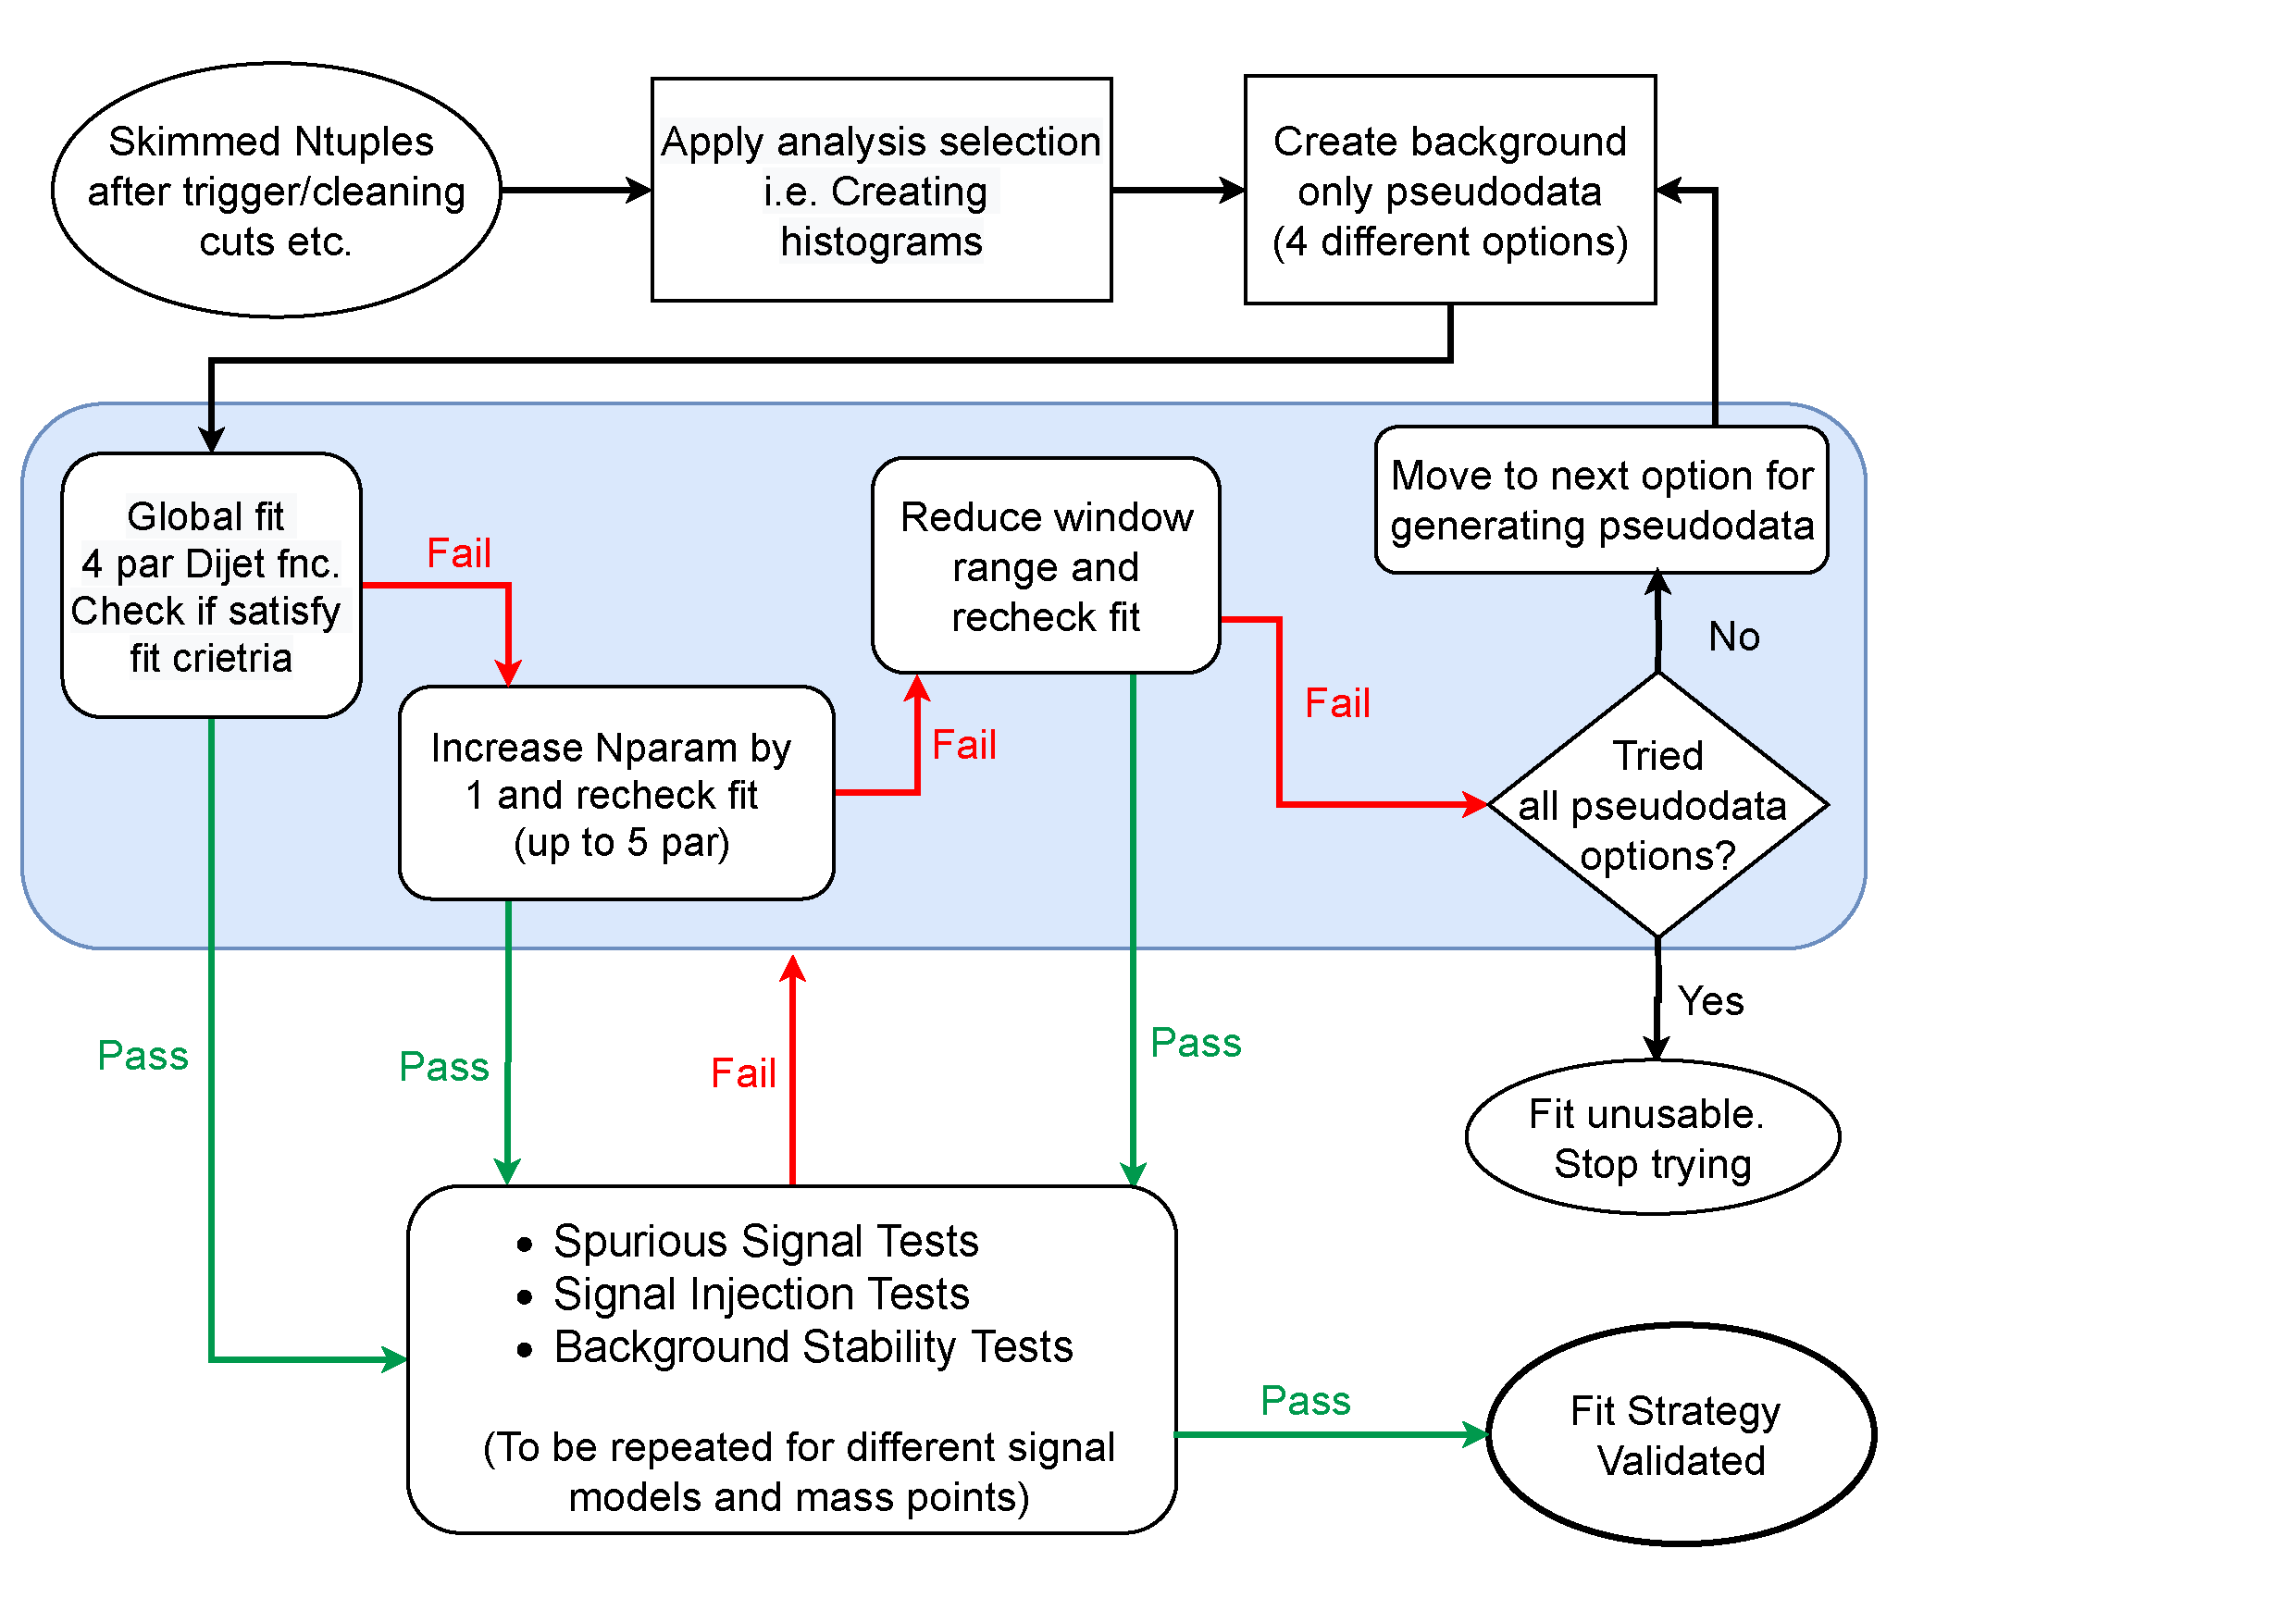
\includegraphics[width=0.75\textwidth]{flowcharts/QGDijet-FlowChart-30March}
\caption{Analysis top-level flowchart.
\label{eflow}}
\end{figure}

The main kinematic variable used to determine the control versus
signal regions for many of the studies is $y^* = (y_1-y_2)/2$, where
$y_1$ and $y_2$ are the rapidities of the two jets.
This variable is primarily used as a topological variable to define a QCD
enhance control region and a possible resonance enhanced signal region.

As in previous dijet analysis, the background is estimated from the
data itself.
Although Monte Carlo background samples are used extensively, they are
not considered accurate enough to be used as the background-only model.
The data has previously been searched for narrow resonances using an
inclusive two-jet selection.
The inclusive dijet spectrum is thus considered as control region for
some of the gluon/quark tagged studies. 

We aim to obtain the following results from the analysis.

\begin{itemize}
\item Search for high-mass resonances in the inclusive, single-gluon tagged,
  and double-gluon tagged dijet systems.
\item If nature is willing, claim something interesting, else set of
  limits. 
\item Set model independent upper-limits on resonance cross sections for
  inclusive, single-gluon tagged, and double-gluon tagged dijet systems.
\item For the string resonance model, set lower limits on the string
  scale for inclusive, single-gluon tagged, and double-gluon tagged
  dijet systems; hopefully, demonstrating the best sensitivity for
  single-gluon tagging.
\item For the H$^\prime$ resonance model, set lower limits on the
  resonance mass for inclusive, single-gluon tagged, and double-gluon
  tagged dijet systems; Hopefully, demonstrating the best sensitivity
  for  double-gluon tagging.
\end{itemize}

%%%%%%%%%%%%%%%%%%%%%%%%%%%%%%%%%%%%%%%%%%%%%%%%%%%%%%%%%%%%%%%%%%%%%%%%%%%%%%%%%%%%%%%%%%%%%
\subsection{Milestones}

\begin{table}[htb]
\caption{Milestones in the analysis.}
\begin{tabular}{llll}\hline
Task & Analyzer & Role & Other responsibilities\\\hline
Milestone 1\\
\color{red}{Generation dijet invariant mass pseudo-distributions} & many & many & others\\
\color{red}{Perform S+B fitting of pseudo-data}                   & many & many & others\\
\color{green}{Unblinding}                                         &
many & many & others\\
\hline
Milestone 2\\
\color{red}{Perform S+B fitting of data}                          & many & many & others\\
\color{green}{Decision to claim discover or set limits}           & many & many & others\\
\hline
Miletone 3\\
\color{red}{Set model-independent limits}                         & many & many & others\\
\color{red}{Set model-dependent limits}                           & many & many & others\\
\hline
Milestone 4\\
\color{green}{Write paper}                                        & many & many & others\\
\hline
\end{tabular}
\end{table}
%%%%%%%%%%%%%%%%%%%%%%%%%%%%%%%%%%%%%%%%%%%%%%%%%%%%%%%%%%%%%%%%%%%%%%%%%%%%%%%%%%%%%%%%%%%%%
